\documentclass{beamer}
\usetheme{Madrid}
\usecolortheme{default}
\usepackage{graphicx}
\usepackage{amsmath}
\usepackage{hyperref}

\definecolor{mycolor}{RGB}{144,180,148}
\setbeamercolor{structure}{fg=mycolor}

\title{An Introduction to Dynamics}
\subtitle{SPH-3UI Grade 11 Physics}
\date{\today}

\begin{document}

\frame{\titlepage}

% Slide 1: Motion
\begin{frame}
\frametitle{Why study dynamics?}
\textbf{Kinematics} studies \textbf{how} objects move.  
It answers questions like how far, how fast, and for how long motion occurs.  

\vspace{0.5cm}
\textbf{Dynamics} studies \textbf{why} objects move the way they do.  
It focuses on the causes of motion — what forces act, why something speeds up, slows down, or changes direction.

\begin{center}
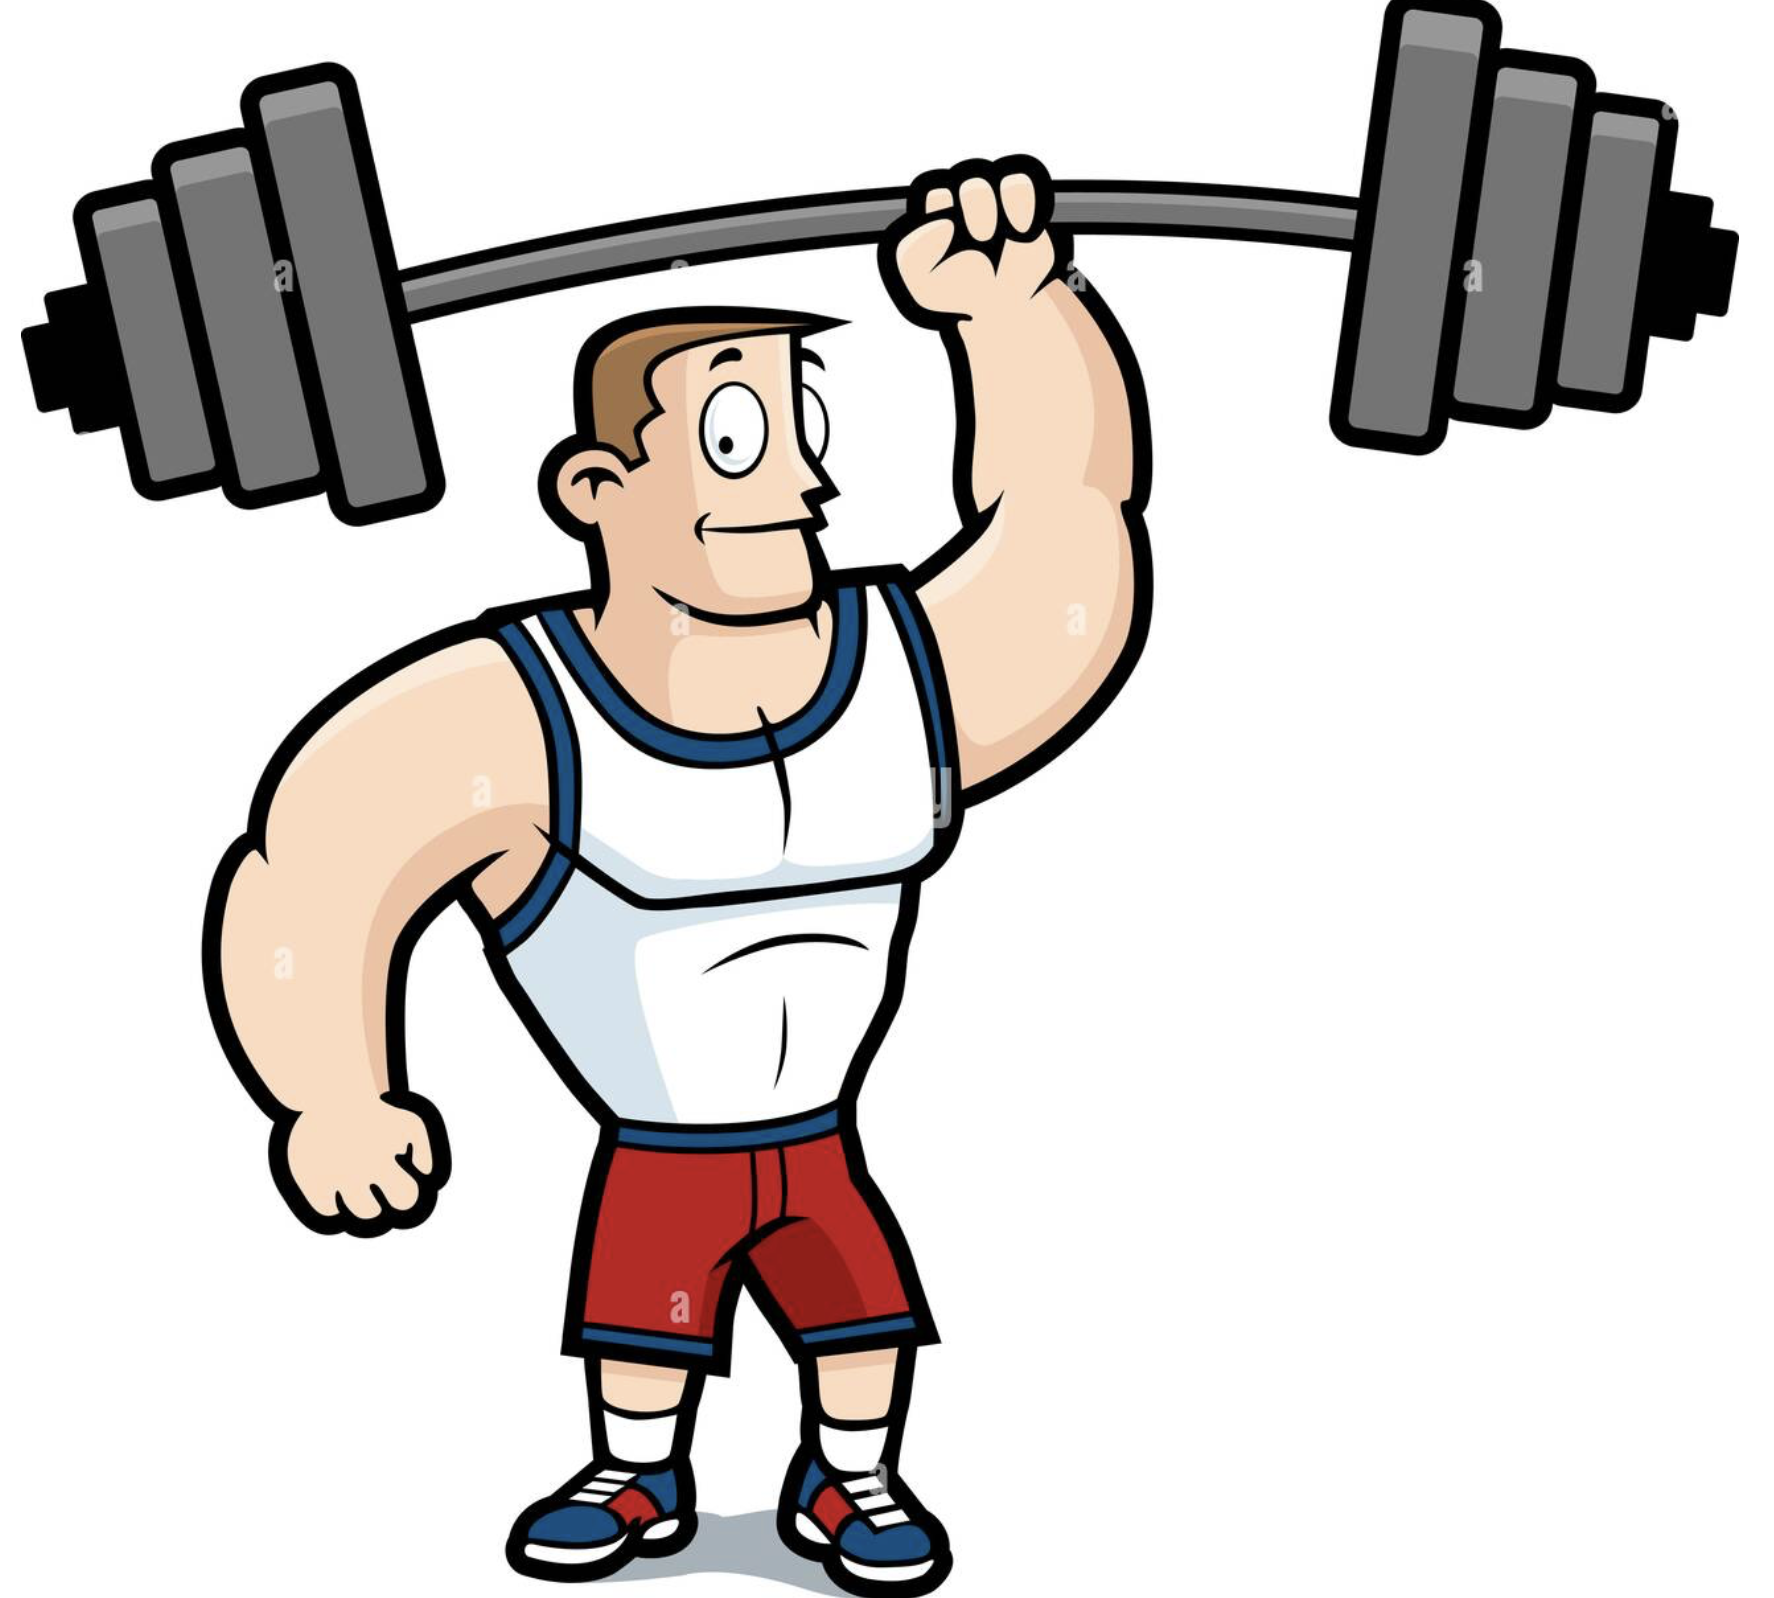
\includegraphics[width=0.4\textwidth]{strongdude.png}
\end{center}

\end{frame}

% Slide 3: What is Force?
\begin{frame}
\frametitle{What is Force?}
\begin{beamercolorbox}[rounded=true, shadow=true, wd=\textwidth, sep=1em]{title}
A force is a \textbf{push} or a \textbf{pull} that can cause an object to change its motion or shape.  

     \end{beamercolorbox}



\vspace{0.3cm}
 In physics, force is represented by a \textbf{vector} because it has both magnitude and direction.  
    For example, pushing a book sideways will have a different effect than pulling it upward.

\vspace{0.3cm}
Forces are the fundamental way that matter interacts with matter.
\end{frame}

% Slide 4: Measuring Forces - The Newton
\begin{frame}
\frametitle{Measuring Forces: The Newton}

\begin{columns}[T]
\begin{column}{0.7\textwidth}
    The SI unit of force is the \textbf{newton (N)}, named after Isaac Newton.  
    One newton is the force required to accelerate a 1 kg mass by 1 m/s\textsuperscript{2}.  
    
    \vspace{0.3cm}
    \textbf{Tools to measure force:}
    \begin{itemize}
    \item A spring scale stretches more with greater pulling force.
    \item A digital force sensor records and graphs force changes over time.
    \end{itemize}
    \end{column}
    \begin{column}{0.3\textwidth}
    \centering
    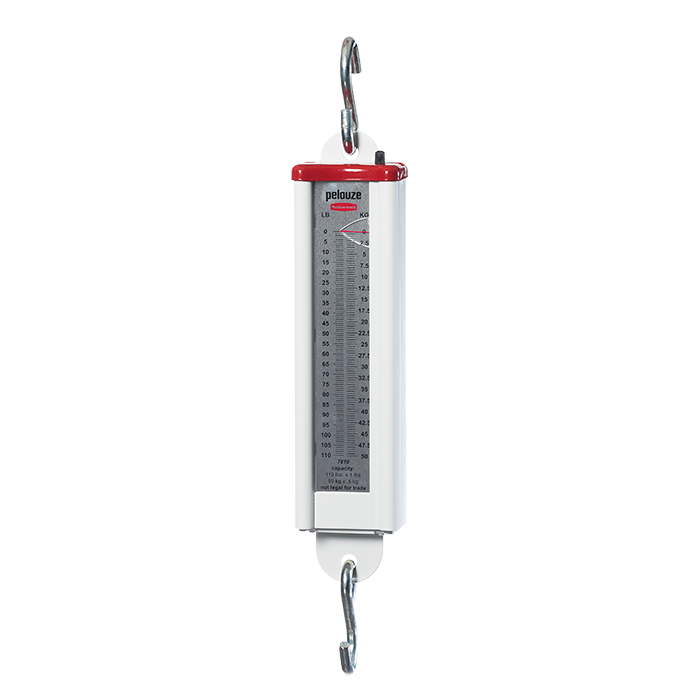
\includegraphics[width=1.3\linewidth]{springscale.png}
  \end{column}
\end{columns}
\end{frame}

% Slide 10: Atoms and Fundamental Particles
\begin{frame}
\frametitle{Atoms and Fundamental Particles}
\begin{columns}
\column{0.5\textwidth}
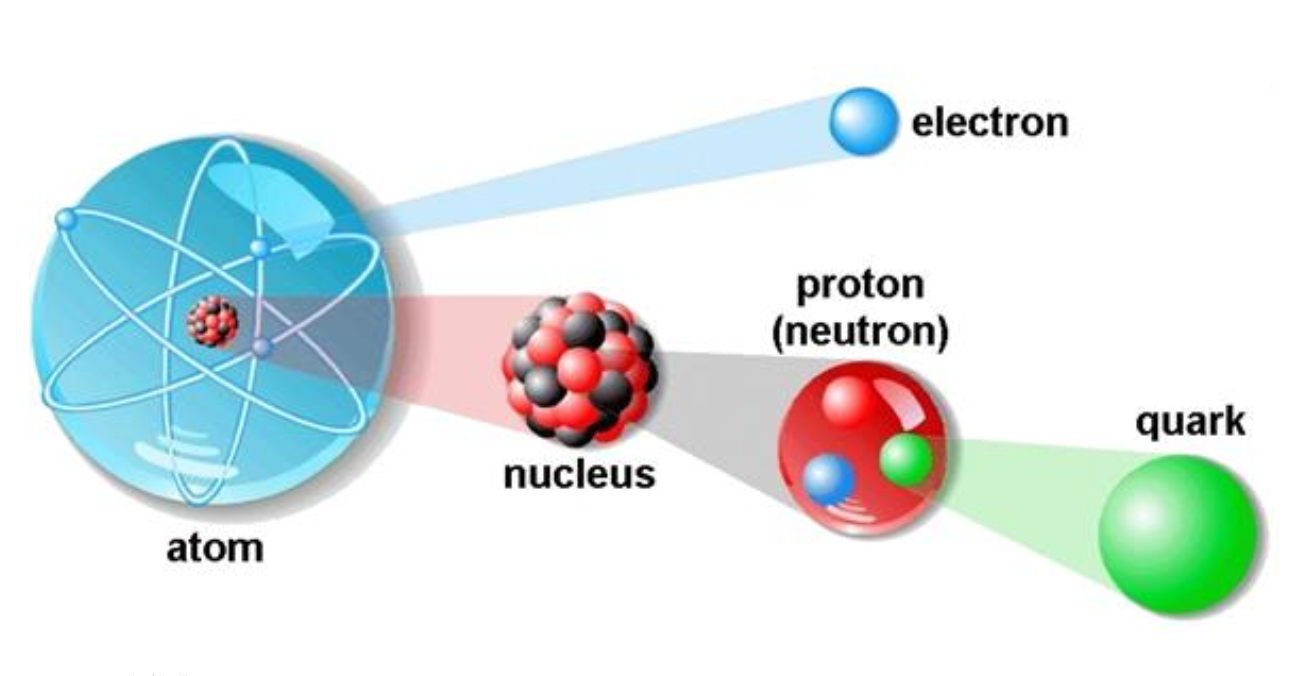
\includegraphics[width=0.9\textwidth]{atom.png}
\column{0.5\textwidth}
Atoms are made of protons, neutrons, and electrons.  
The electron is a fundamental particle called a lepton.  
Protons and neutrons are made of smaller particles called quarks:
\begin{itemize}
\item Proton: 2 up quarks + 1 down quark.
\item Neutron: 2 down quarks + 1 up quark.
\end{itemize}
\end{columns}
\end{frame}

% Slide 5: The Standard Model
\begin{frame}
\frametitle{The Standard Model}
The \textbf{Standard Model of Particle Physics} is our best theory for explaining the fundamental building blocks of the universe.  

It divides all particles into two main types:
\begin{itemize}
\item \textbf{Fermions:} particles that make up matter (quarks and leptons).
\item \textbf{Bosons:} particles that carry forces (photons, gluons, W and Z bosons, etc.).
\end{itemize}

\begin{center}
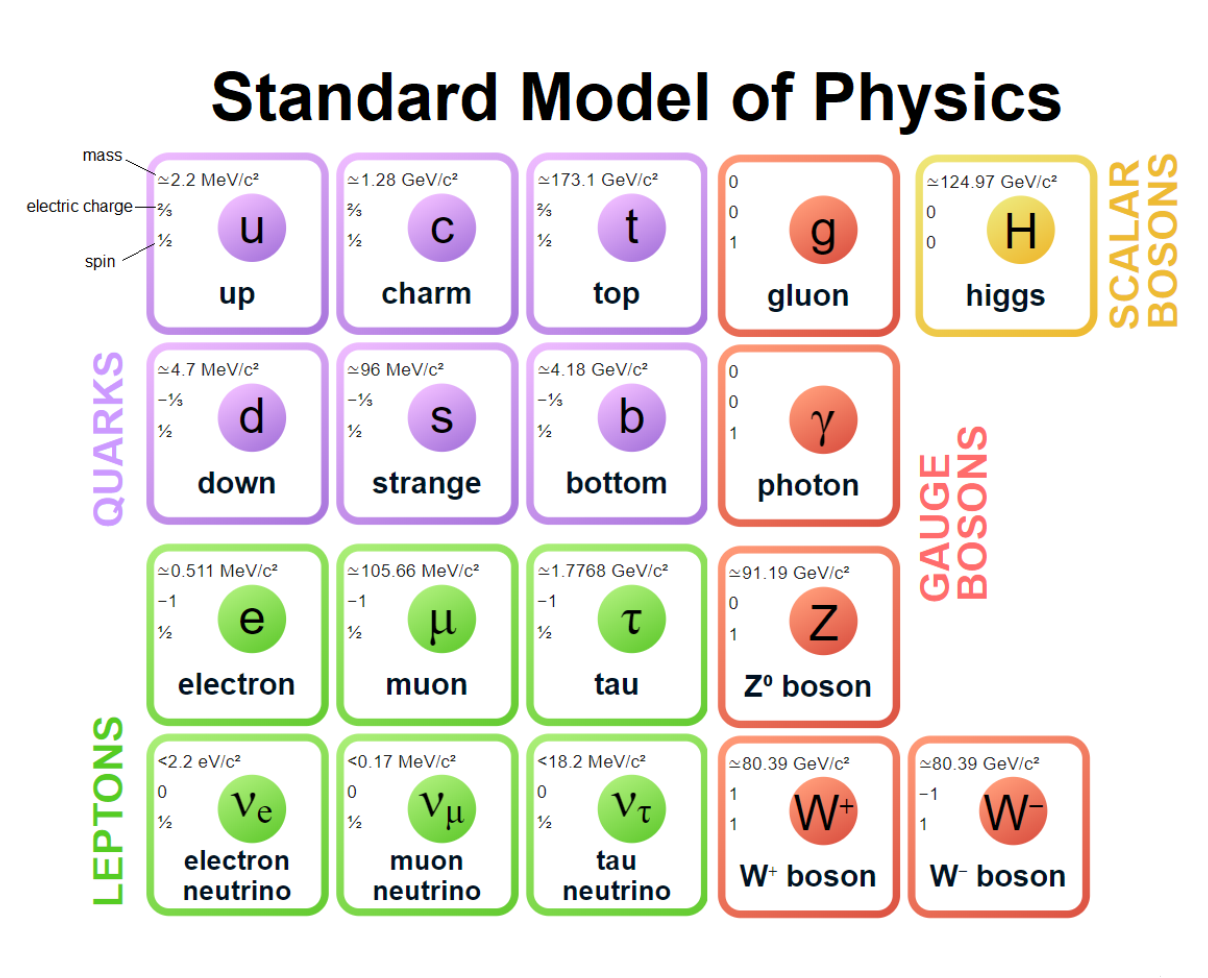
\includegraphics[width=0.5\textwidth]{standardmodel.png}
\end{center}
\end{frame}

% Slide 14: Videos
\begin{frame}
\frametitle{Watch These!}
\begin{center}
\href{https://youtu.be/Unl1jXFnzgo?si=SVN_GrBsFqQ8xlAg}{\textbf{The Standard Model: A Triumph of Science}}\\[0.5cm]
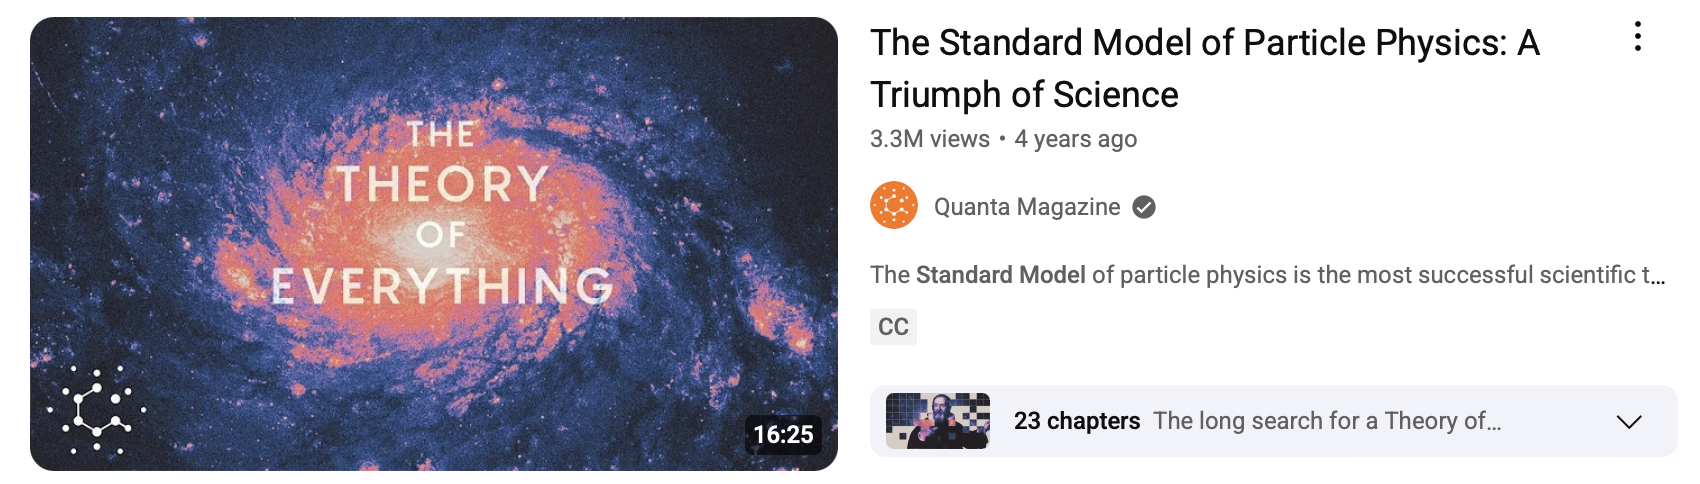
\includegraphics[width=1.0\textwidth]{standardmodelvideo.png}
\end{center}
\end{frame}

% Slide 6: Gauge Bosons and Forces
\begin{frame}
\frametitle{How Do Particles Exert Forces?}
Forces occur through the exchange of \textbf{gauge bosons}, the messenger particles of nature.  

\vspace{0.3cm}
When two electrons repel each other, they’re constantly exchanging photons.  
This transfer of momentum is what we experience as a force.  

\vspace{0.3cm}
Imagine two people in rolling chairs tossing a medicine ball.  
Each slides backward when the ball is thrown or caught.  
The ball acts like a photon, carrying the force between them.

\begin{center}
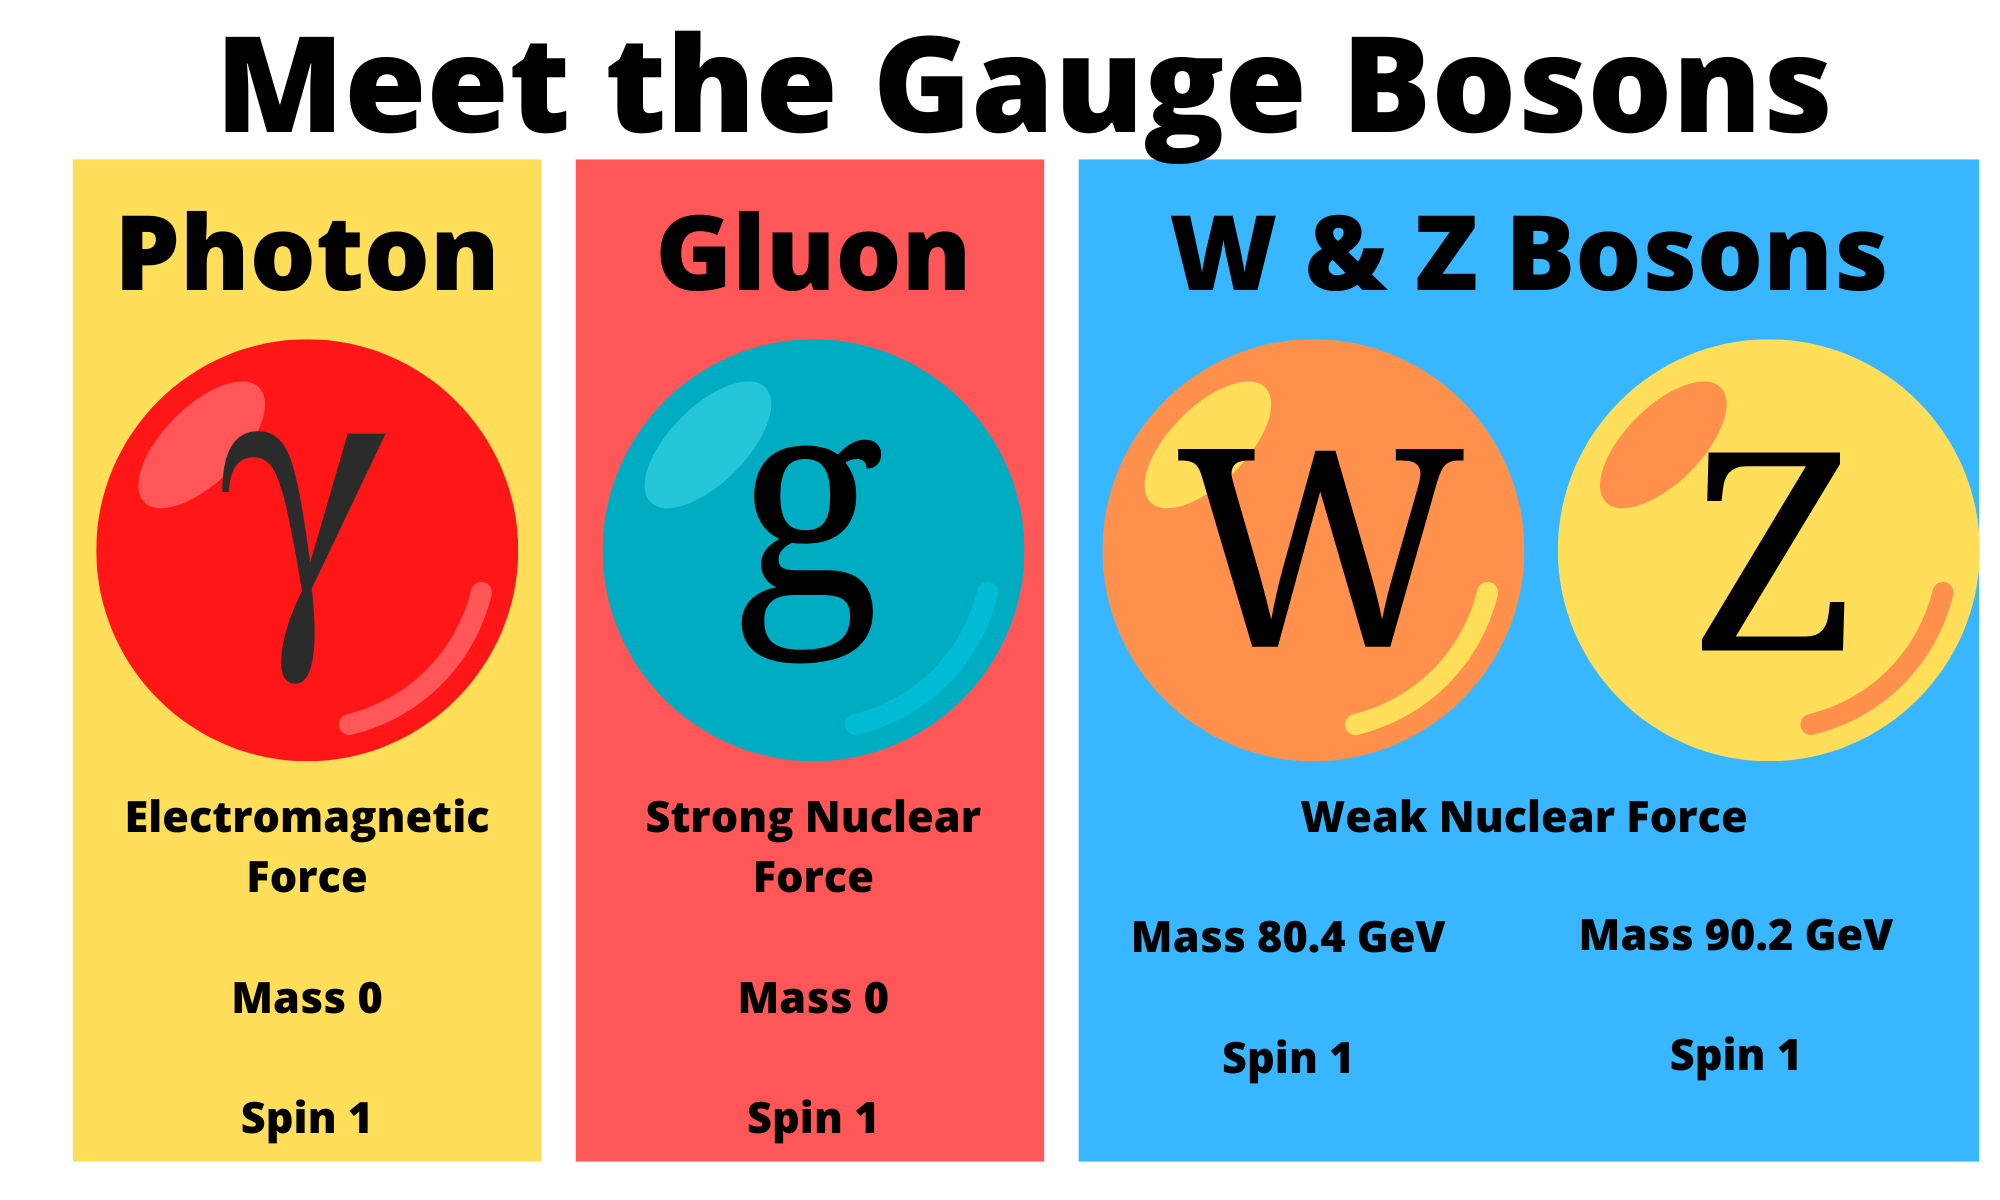
\includegraphics[width=0.4\textwidth]{gaugeboson.png}
\end{center}
\end{frame}

% Slide 7: The Four Fundamental Forces
\begin{frame}
\frametitle{The Four Fundamental Forces}
All interactions in the universe can be explained by four fundamental forces:
\begin{itemize}
\item \textbf{Gravitational Force:} acts between masses; always attractive.
\item \textbf{Electromagnetic Force:} acts between charged particles; can attract or repel.
\item \textbf{Strong Nuclear Force:} binds protons and neutrons inside the nucleus.
\item \textbf{Weak Nuclear Force:} responsible for radioactive decay and particle transformations.
\end{itemize}

\centering
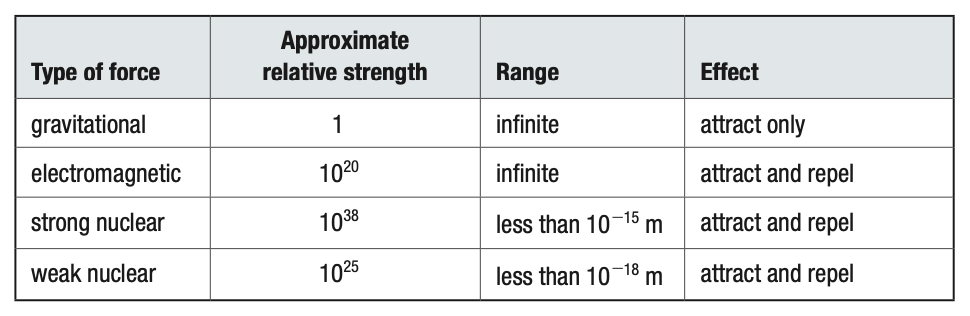
\includegraphics[width=\linewidth]{FFtable.png}

\end{frame}

% Slide 9: Why the Standard Model is Incomplete
\begin{frame}
\frametitle{Why the Standard Model is Incomplete}
Although extremely successful, the Standard Model does not explain everything.  
It leaves out gravity, dark matter, and dark energy.  

\vspace{0.3cm}
Some unanswered questions:
\begin{itemize}
\item Why are there three families of quarks and leptons?
\item Why do particle masses vary so much?
\item What gives particles their mass? (Answered in 2012!)
\item How does gravity fit with the other forces?
\end{itemize}

Scientists are searching for a \textbf{Grand Unified Theory (GUT)} or even a \textbf{Theory of Everything (TOE)}.
\end{frame}




% Slide 10: Everyday Forces
\begin{frame}
\frametitle{Everyday Forces}


Example: A wagon is being pushed and pulled by two children. 

\begin{center}

Which forces are acting on the wagon? 

\vspace{0.3cm}

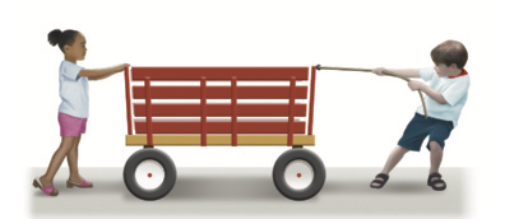
\includegraphics[width=0.9\textwidth]{wagon.png}
\end{center}


\end{frame}

% Slide 11: Everyday Forces
\begin{frame}
\frametitle{Everyday Forces}
Objects experience many familiar forces:
\begin{itemize}
\item \textbf{Applied Force ($\vec{F}_{A}$):} push or pull from contact.
\item \textbf{Tension ($\vec{F}_T$):} pull from a rope or string.
\item \textbf{Normal Force ($\vec{F}_N$):} upward support from a surface.
\item \textbf{Friction ($\vec{F}_f$):} opposes motion along a surface.
\item \textbf{Gravity ($\vec{F}_g$):} attraction due to mass.
\end{itemize}

\begin{center}
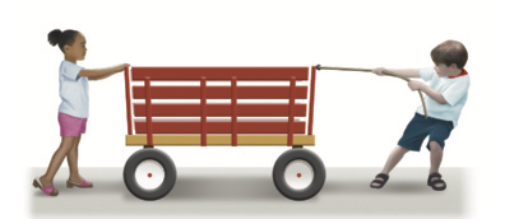
\includegraphics[width=0.5\textwidth]{wagon.png}
\end{center}

\end{frame}

% Slide 12: Free-Body Diagrams
\begin{frame}
\frametitle{Free-Body Diagrams (FBDs)}
To analyze motion, we draw a \textbf{free-body diagram} (FBD).  
It shows an object and all the forces acting on it.  

\begin{itemize}
\item Draw the object as a box or dot.
\item Represent each force with an arrow pointing away from the object.
\item Longer arrows represent larger forces.
\item Label each force ($\vec{F}_N$, $\vec{F}_g$, etc.).
\end{itemize}
\vspace{-0.2cm}

\begin{center}
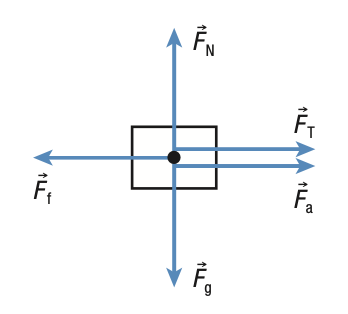
\includegraphics[width=0.5\textwidth]{FBD.png}
\end{center}
\end{frame}

% Slide 13: Net Force
\begin{frame}
\frametitle{Net Force}
Once all forces are identified, they combine to form a single \textbf{net force}.  

\[
\vec{F}_{net} = \sum \vec{F}
\]

The net force determines the object’s acceleration:
\[
\vec{F}_{net} = m\vec{a}
\]

If the net force is zero, the object remains at rest or moves at constant velocity.
\end{frame}

% Slide 12: Free-Body Diagrams
\begin{frame}
\frametitle{Example 1: Free-Body Diagrams (FBDs)}


\begin{beamercolorbox}[rounded=true, shadow=true, wd=\textwidth, sep=0.5em]{title}
\begin{itemize}
\item Draw the object as a box or dot.
\item Represent each force with an arrow pointing away from the object.
\item Longer arrows represent larger forces.
\item Label each force ($\vec{F}_N$, $\vec{F}_g$, etc.).
\end{itemize}
\end{beamercolorbox}

\vspace{0.8cm}
\noindent
Try the following examples: 
\begin{itemize}
    \item A cup sitting at rest on a table. 
    \item A large trunk in the basement is pulled by a rope tied to the right side of the trunk by a person. The trunk does not move. 
    \item A baseball player is sliding to the left across the ground. 
    \item A desk is pushed to the left across the floor. 
\end{itemize}
\end{frame}

\end{document}
